\documentclass[10pt,twocolumn,letterpaper]{article}

\usepackage{cvpr}
\usepackage{times}
\usepackage{epsfig}
\usepackage{graphicx}
\usepackage{amsmath}
\usepackage{amssymb}
\usepackage{subfigure}% in preamble

% Include other packages here, before hyperref.

% If you comment hyperref and then uncomment it, you should delete
% egpaper.aux before re-running latex.  (Or just hit 'q' on the first latex
% run, let it finish, and you should be clear).
\usepackage[breaklinks=true,bookmarks=false]{hyperref}

\cvprfinalcopy % *** Uncomment this line for the final submission

\def\cvprPaperID{****} % *** Enter the CVPR Paper ID here
\def\httilde{\mbox{\tt\raisebox{-.5ex}{\symbol{126}}}}

% Pages are numbered in submission mode, and unnumbered in camera-ready
%\ifcvprfinal\pagestyle{empty}\fi
%\setcounter{page}{4321}
\DeclareMathOperator*{\argmax}{arg\,max}
\begin{document}

%%%%%%%%% TITLE
\title{Diminished Triad: Consistent Hashing in Redis}

%% TODO: Have to figure out how to add multiple authors
\author{Pallavi Agarwal, Manindra Kumar Moharana, Sanjeev Jagannatha Rao\\
University of California, San Diego\\
%\small PID: A53068263\\
\small p1agarwa,mmoharana,sjrao@ucsd.edu}

% For a paper whose authors are all at the same institution,
% omit the following lines up until the closing ``}''.
% Additional authors and addresses can be added with ``\and'',
% just like the second author.
% To save space, use either the email address or home page, not both


\maketitle
%\thispagestyle{empty}


%%%%%%%%% BODY TEXT
\section{Abstract}
Diminished Triad is a (partial) diminished implementation of chord by the three authors on Redis backends. Redis is an open source, BSD licensed, advanced key-value cache and store.
While Redis offers an extremely fast key value cache, its design suffers from some major drawbacks. Redis does not support consistent hashing, the slaves of a particular master are only aware of the master that they are replicating and unaware of the state of the rest of the system. Redis also does not support automatic migration of keys when a new node joins or readjustment of responsibilities when a node fails. Diminished Triad aims to address these drawbacks of Redis at the cost of an additional layer of indirection and its associated overheads.

\section{Introduction}
``Redis is an open source, BSD licensed, advanced key-value cache and store. It is often referred to as a data structure server since keys can contain strings, hashes, lists, sets, sorted sets and bitmaps"\cite{redis} . Twitter, GitHub, Weibo, Pinterest, Snapchat, Craigslist, Digg, StackOverflow and Flickr are some of the well known companies currently using Redis. Redis prides itself on providing very fast performance and several of its design choices have been made with this primary objective. For example, Redis supports asynchronous master slave replication. However, if the master dies before the data is replicated to the slaves, that piece of data is lost. Redis backends are also either only a slave or master and can not be both. A slave replicates a particular master and is unaware of the rest of the system. If a Redis system has r backups, it can support at most r random node failures. If we loose a master and all its slaves we loose all the master's data. Redis contains 16348 key slots. Every key maps to one of these key slots. Redis does not support consistent hashing. When a system is started all the key slots are evenly distributed among the masters.  When a new node joins the system, keys need to be migrated manually to the new node.

In order to achieve its outstanding performance, Redis works with an in-memory dataset. So it offers very high write and read speeds with the limitation that data sets can't be larger than memory. Being an in memory dataset, Redis can work with complicated data structures and supports several of them with very little internal complexity. Redis can persist data by either dumping the data to disk every once in a while, or by appending each command to a log. We have adopted the latter approach with our Redis backends as it works like a redo log to migrate data when a new node joins the system. 

In Diminished Triad (DT), we hope to provide a fault tolerant systems using Redis backends that improves on several drawbacks of the existing Redis system described earlier. First,  DT follows a consistent hashing system similar to Chord \cite{chord}. It hashes every backed and keys to a position on the ring. Second, DT automatically moves keys between nodes every time a node joins or leaves the system. Third, DT system, like chord is completely distributed and no node is more important that the other. 

DT maintains two invariants:
\begin{enumerate}
  \item Each node is the master for all the keys that hash between its predecessor and itself.
  \item All the data that a node is responsible for (keys for which it is the master) are replicated in the r nodes next to it on the ring (in clockwise order).
\end{enumerate}
Every node is thus a master for some of the keys and is a backup for the r nodes that precede it. Every time a node is added to the system or a node fails and leaves the system, the keys are redistributed amongst all the backends to maintain the two invariants.

The rest of the paper is organized as follows. Section \ref{design} contains the detailed design of Diminished Triad. This section mentions the various components of DT, their individual roles, the APIs used to communicate between these components. Section \ref{implementation} provides the implementation details of DT. Section \ref{evaluation} provides various metrics that measure the performance of Diminished Triad. This section discusses the relative merits and demerits of Diminished Triad over off the shelf Redis.


\section{Design} \label{Design}
We first define several terms that will be helpful in describing the system. 

\begin{enumerate}
  \item User/Client - A user or a client is the customer for the Diminished Triad service. For example, a client requests to set values for some keys, get values etc.
  \item DTServer - All requests like get and set are made by the client to the DTServer. The DTServer then forwards the request to the appropriate backends that are responsible for the key being queried through the DTClient
  \item DTClient - The DTClient is the only channel of communication with the Redis Backend. The DT client transforms the requests received by the DTServer into form understandable by the Redis Backend and queries the appropriate Redis Backend.
  \item DTInstance - DTInstance comprises of the DTServer and a pool of DTClient instances
  \item Redis Backend - This is the off the shelf Redis Server instance that provides all the key value store functionality to Diminished Triad.
  \item DTClientAPI - The user talks only to the DT instance and is unaware of the intricacies of the system. From the user's perspective the DT instances provide a fault tolerant distributed key value store. The DTClientAPI defines all the functions exported by the DTServer to the client. This API makes hides the internal details of DT and makes it look like a fault tolerant key value store to the programmer. A list of all the functions exported DTClientAPI is mentioned later. 
  \item DTServerAPI - The DTInstance, in particular the DTClient talks to the Redis Backends though a set of functions exported by the Redis Backend. This API is completely internal to the DTInstance and the user is completely unaware of the DTServerAPI.
  \item Sentinel - The sentinel is the watchdog for the Redis Backends. It actively monitors if the Redis Backends are working as expected. The Sentinel also notifies through an API when something is wrong with one of the monitored Redis instances.
   \item DTSentinel -  The DTSentinel listens to notifications from the sentinel for any changes like a node leaving the system or joining the system and takes appropriate action in each case to maintain the DT system invariants.
\end{enumerate}



\subsection{System Layout}
Every node runs a Redis Backend and a DTInstance. All DTInstances are identical and none of them are more important than the other. A client can talk to any DTInstance using the DTClientAPI. The DTClient will forward the request to the appropriate Redis Backend using the DTServerAPI. Note that the Redis Backend servicing the client's request may or may not be on the same machine as the DTInstance.
At the moment we have a single Sentinel and DTSentinel instance in our system. We can make our system tolerant to failures of the Sentinel and DTSentinel with minor configuration changes to the Sentinel configuration. The section \ref{fwork} on future work briefly mentions how this can be accomplished. Without loss of generality we will be discussing the system with just one instance of Sentinel and DTSentinel and assume them to be free from failure. Figure \ref{design} shows a typical set for Diminished Triad.

\begin{figure*}[htb]
  \centering
  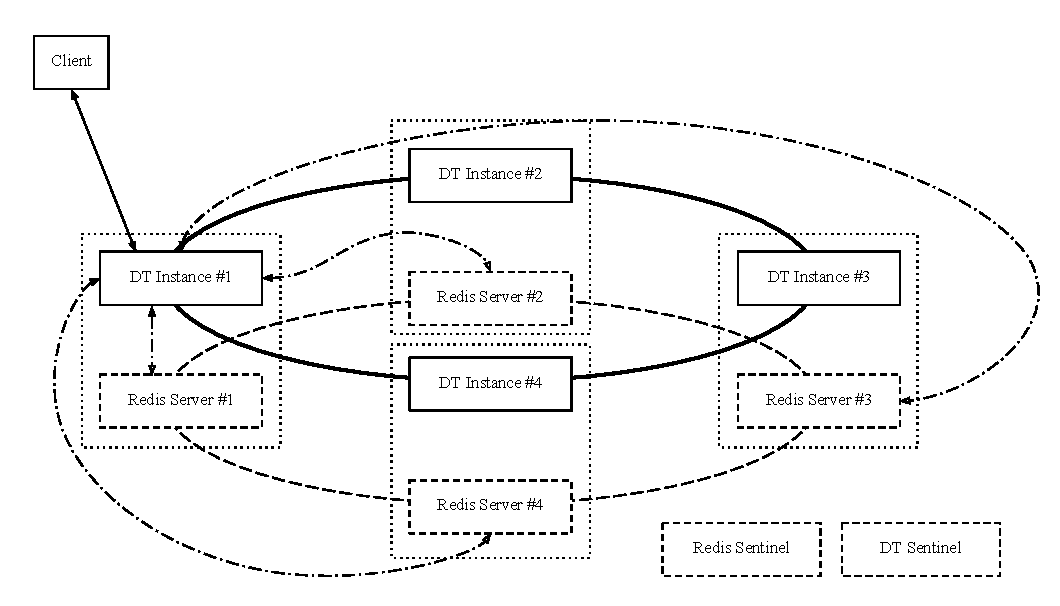
\includegraphics[scale=0.75]{impl3.pdf}
  \caption{System Design. The solid lines represent the parts visible to the user. The dashed lines represent the parts hidden from the user.}
\end{figure*}

\subsection{DTClientAPI}
Diminished Triad exposes the following functions to the user. This is a subset of the functions exported by the Redis Backend in the DTServerAPI. A complete implementation of Diminished Triad will ideally expose every single function exported by the Redis Backend. We have limited our scope to the functions listed below.
\begin{itemize}
  \item get(key) - gets the value associated with a particular key
  \item set(key,value) - set the value associated with a particular key
  \item getStrlen(key) - get length of a value associated with a particular key
  \item append(key,value) - append a value to the value already associated with a particular key
  \item lPush(key,value) - insert a value in the first position to the list associated with a particular key
  \item lPop(key) - remove and return the first element of the list associated with a particular key
  \item lIndex(key,index) - return the element at a particular index in the list associated with a particular key
  \item lLen(key) - get length of list associated with a particular key
\end{itemize}

\subsection{The Chord Ring, Hashing Keys, Master and the R Backups}
The Chord ring has N positions in it. Every node hosting a DTInstance and a Redis backend is hashed to one of these N positions. Every key is also hashed to one of these N positions. As we move clockwise in the chord ring, we encounter increasing values of hash values until we reach the maximum and then go back to 0. Every backend is the master for the all the keys that hash to its position in the ring through the hash positions up to but not including its  predecessor in the ring. The predecessor of a backend is defined as the first live backend that is encountered as we move anti clockwise in the chord ring. Similarly the successor is the first live backend that is encountered as we move clockwise in the chord ring. The r backends that immediately succeed the master serve as the r backups of that particular master. 

\subsection{Handling Read and Write Requests}
A read or write request is issued by the user or client to the DTInstance. The request reaches the DTServer running in the DTInstance through the DTClient API. The DTServer receives the request, hashes the key to figure out the master and the r backups corresponding to the key. It then performs the actions required for the request on the  r + 1 redis backends (mater plus the r backups) using the DTClient to connect to them which implements the DTServerAPI to talk to the redis backends. If the request is a write request, the DTInstance writes synchronously to the master and all the backups. If it is a read request, the DTInstance returns on the first successful read starting with the master and then trying the r backups.


\subsection{The Sentinel, DTSentinel}
The Sentinel is a watchdog for all our Redis backends. In Diminshed Triad, we use the Sentinel for performing the following:
\begin{itemize}
  \item Monitoring - Sentinel constantly checks if the Redis Backends are working as expected
  \item Notification - Sentinel notifies the DTSentinel thorough pub/sub messages that something is wrong with one of the monitored Redis Backends.
  \item Configuration provider - The sentinel maintains the configuration of all the currently alive Redis Backends.
\end{itemize}

The Sentinel itself is designed to run in a configuration where there are multiple Sentinel processes cooperating together. We have not configured our Sentinel to work this way but this can be accomplished with minor configuration modifications. These changes make the Sentinel fault tolerant to failures. 

The DTSentinel listens to notifications from the Sentinel. Every time a node fails or a new node joins, the DTSentinel receives the notification from the Sentinel and is responsible for redistributing data and maintaining the two Diminished Triad invariants. The next section describes how data is moved when a node fails or a new node joins the system.

\subsection{Data Resharding for new/failed nodes}

Whenever an existing node fails or a new node joins the ring, our system performs automatic data resharding. This is significant improvement over the redis cluster system. In redis cluster, redis-trib utility is used to add new nodes. The redis-trib utility provides the system administrator to manually move hash slots from an existing node to the new node. Redis cluster does not offer any automation for this process. The sections below explain the resharding mechanism when a node fails or a new node joins in diminished triad. 

\subsubsection{Node Failure} 
Figure \ref{handledead} shows the resharding steps when a redis backend fails. For the purposes of this section, we assume our system is configured to have two backups for every master. The initial configurations of the system is shown inside the chord ring. M represents a particular master, B1 and B2 its two backups, M-1 and M-2 its two predecessors. In the figure, M is assumed to have failed. The new configuration after M fails is shown outside the chord ring. In order to get to the configuration and maintain the two Diminished Triad invariants, we need to perform 3 data migrations. In general, if we have r backups, we need to perform r + 1 data migrations. Each of these data migrations is shown by an arrow in figure \ref{handledead}. The arrow originates along a section of the chord ring and terminates at a redis backed. The arrow indicates that a copy of all the keys that are hashed to that section of the chord ring have to be migrated to the redis backed that the arrow is pointing to from a redis backend that has all the keys that are being migrated in a consistent state. For example, when M fails, we will move keys for which it was the master , i.e. the keys that originally hashed between M and M-1 to redis backend B2. Since B1 was originally a backup of M, it will have this data and all this data will be migrated from the original B1 to the new reconfigured B2. This data migration is shown by the arrow A2 that originates between the original M and original M-1 redis backends. Similarly we move data corresponding to each arrow A1, A2 and A3. Once data migrations is completed, the Diminished Triad invariants are guaranteed to be restored after the node failure.

\begin{figure}[hbt]
  \centering
  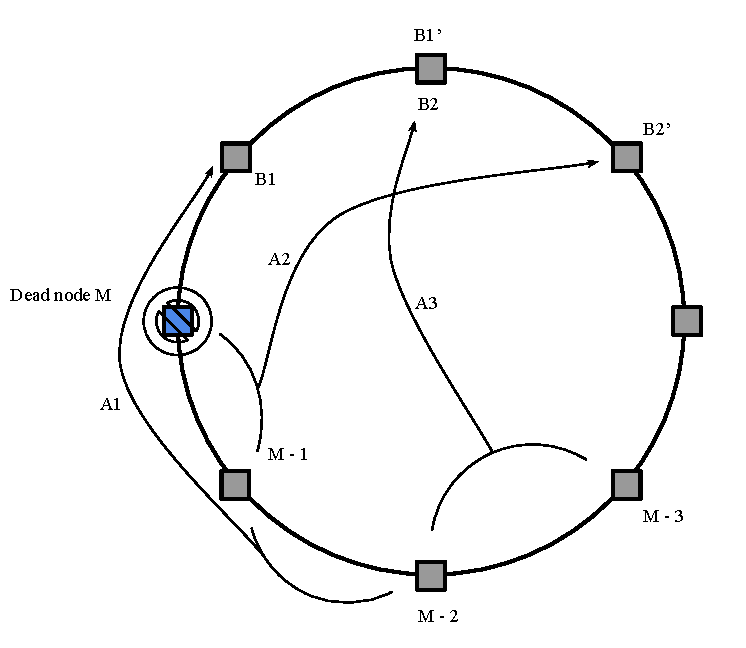
\includegraphics[scale=0.6]{handle_dead.pdf}
  \caption{Data Migration During Failures}
  \label{handledead}
\end{figure}

\subsubsection{Node Join} Similarly, when a node joins, if the system is configured to have r backups,  a set of r+1 data migrations is sufficient to bring the node into the system and restore the Diminished Triad invariants. As in the previous section, assume the system is configured to have two backups for every master for the rest of this discussion. Figure \ref{handlejoin} shows the data migration that is carried out when a new node joins. Th new node M is the master for all the keys that are hashed between M and M-1. B1 was the master for these keys before M joined. This data is hence moved from B1 to M. This is indicated by the arrow A1 in figure \ref{handlejoin}. 

Additionally, the new node M also servers the first backup for M-1 and the second backup for node M-2. Data for which node M-1 is the master is moved from node M-1 to node M. This is indicated by arrow A2 in figure \ref{handlejoin}. Data for which node M-2 is the master is also moved from node M-2 to node M and this indicated by arrow A3 in figure \ref{handlejoin}.

\begin{figure}[hbt]
  \centering
  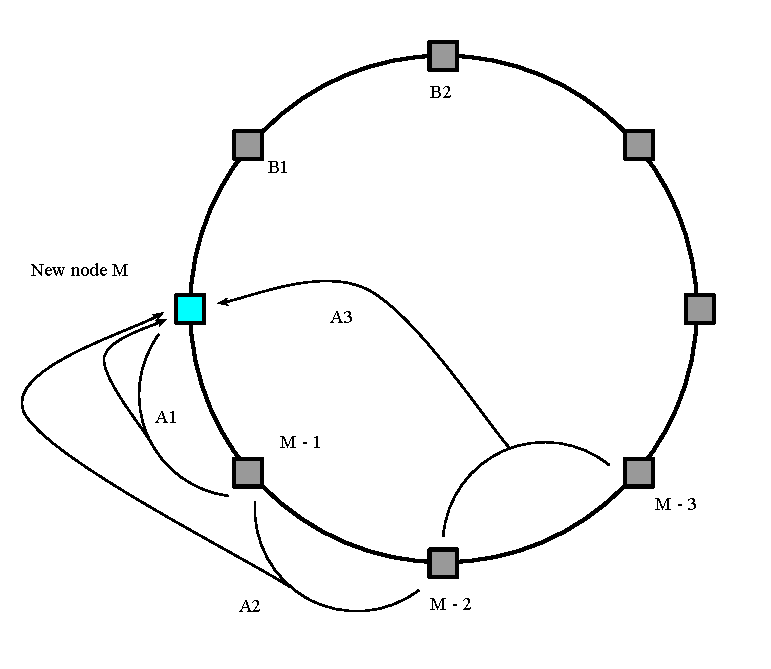
\includegraphics[scale=0.6]{handle_join.pdf}
  \caption{Data Migration During Node Join}
  \label{handlejoin}
\end{figure}


\subsubsection{Handling Writes During Resharding} Redis can persist data by either dumping the dataset to disk every once in a while, or by appending each command to a log. We use the log generated by redis to check if there have been any writes while the data is being migrated. Any new entry in the log implies a new write. All these changes are applied and the migration is deemed complete only when there are no more changes to apply. A new node is allowed into the system only after migration is complete. This method has certain drawbacks. First, an adversary can tailor its writes to target a specific backend by selecting specific keys and can delay a node from joining the system. Second, any write that occurs between the last comparison of the logs to the time the new node joins the system can cause issues. Due to lack of time we did not remedy this issue as it is a rather unlikely event. However, we suggest some methods to handle this issue in the section \ref{futurework} on future work.



\section{Implementation} \label{implementation}
% DT_Server, DT Sentinel, redis-py, spyne


We used Python 2.7 to implement the DT Server, DT Client and DT Sentinel. Python was chosen because of its flexibility and ability to prototype and iterate faster. 

\textbf{DT Server:} Each DT Server functions as a RPC server. We use the spyne rpc toolkit for python to create the RPC server. For each function in the DTClient API (get, set, append, etc.) there's a corresponding RPC function call along with the necessary parameters. RPC calls can be made by HTTP post requests, passing in the redis command and parameters as the post arguments. A DT Server has a upto date list of alive nodes in the ring. When a get/set command is received for a particular key, the server hashes the key and finds out which redis server the key is mapped to. It then forwards the request to the particular server and its backup using DT Client.

\textbf{DT Client: }This the component that talks to the redis servers. Each DT Client is connected to all the redis servers in the ring. We use the redis-py python library for redis. It greatly simplifies the process of talking to a redis server by exposing all redis commands via easy to use API. When the DT Client receives a request for issuing a command for a redis server, it issues the command with the help of redis-py.

\textbf{DT CLI:} To make it easy for the user to send commands to redis, we also designed a utility DT CLI which provides similar behaviour as redis-cli. User can input redis commands like set foo bar, get foo, etc. These commands are converted into a http request and sent to the DT Server. 

\textbf{DT Sentinel:} The DT Sentinel runs in a separate process. Its task is to monitor any configuration changes in the ring and update all the active nodes about the latest configuration. The DT Sentinel is backed by the redis sentinel which is a special sentinel mode of operation of a redis server. In sentinel mode, a redis server doesn't store any key data but monitors other redis servers and can send push notifications on configuration change. DT Sentinel starts up a redis sentinel and subscribes to status change notifications. Any time a node leaves or joins the ring, DT sentinel gets the message from redis-sentinel. DT Sentinel then performs any necessary data migration between nodes and finally sends the latest node configuration to all nodes in the ring.

Data Migration details: 

New node joins


Deploying on AWS:

We tested our system on Amazon AWS. We created 4 instances with 1 GB RAM, 2.2 GHz CPU, running Debian. We started 3 redis servers and instances on each of the machines, redis sentinel  and DT Sentinel on our local machine. We had written scripts which would install all dependencies and dt instances to automate the entire installation process.

We also wrote scripts for evaluating the performance of the system. These scripts wrote random keys and values and measured the latency/consistency with varying values of num-backups, num-servers, etc.


\section{Evaluation} \label{evaluation}

\subsection{Comparison with Redis}
\begin{figure}[hbt]
 \centering
 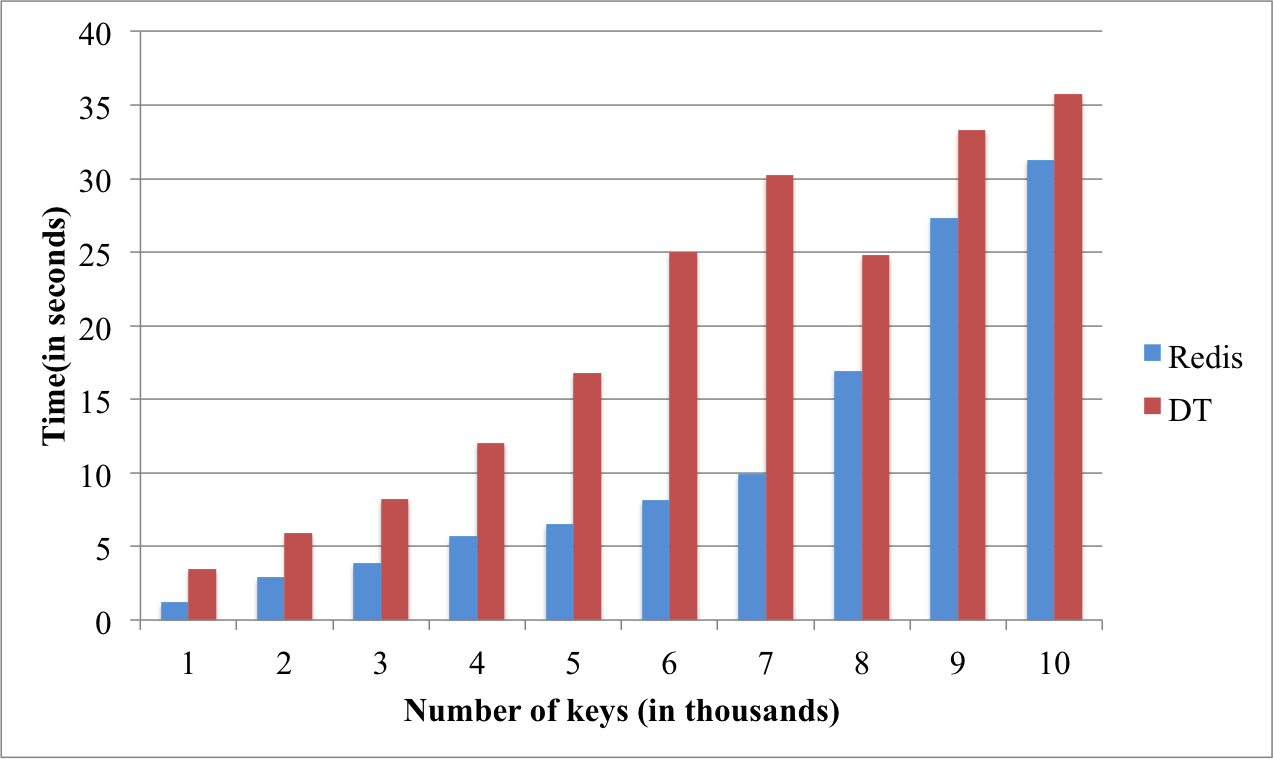
\includegraphics[scale=0.36]{bar_graph}
 \caption{Time taken for 'set' operations on Redis vs DT}
 \label{redisvsDT}
\end{figure}

We performed the \textit{set} operation on both Redis and DT for a number of keys.The setup consisted of 10 Redis servers, 3 backups in case of DT and no slaves. We used the Redis-py library to connect to the Redis backends. The results for the experiment are shown in Fig.\ref{fig:redisvsDT} and it can be seen that the time taken by DT is more than than the time taken by Redis. We identified 3 main reasons for the overhead of 40\% that DT incurs:\\
\begin{enumerate}
 \item DT has an additional layer through which all requests are routed to the correct server. In case of Redis, the client is sent a \textit{redirect} message to the client. This message consists of the address for a different server which has the hash slot to which the key should be mapped. The client then reissues the request to the new server and the set completes. Even though there may be a redirect issued in this case, transfer of messages between instances in case of DT and marshalling and unmarshalling the request result in an overhead.
 \item The Redis-py library has a class called ConnectionPools which manages a set of Connection instances and it ships with two types of Connections. The default, Connection, is a normal TCP socket based connection. The UnixDomainSocketConnection allows for clients running on the same device as the server to connect via a unix domain socket. Since we have no such provision in case of DT, we require new connections to the servers every time we service a request. A Connection Pool-like optimization would reduce the overhead when consecutive requests are made in a short span of time.
 \item In Redis, if a master dies immediately after a write is performed on the master but the background process has not yet synchronized this write with the slaves, the data is lost. We tried to address this problem by synchronously performing the writes on all backups and then returning a response to the client. To counter this, we could write to logs first and then simultaneously write to all servers(primary and backups) using a background process, similar to the one that Redis has. The lack of slaves set up for this experiment have no impact for Redis because the updates to slaves are made asynchronously and the measured time would not change.
\end{enumerate}


\subsection{Comparing Fault Tolerance and Probability of Losing Data between DT and Redis}
Consider a system with \(N\) nodes and \(r\) backups. Assuming infinite capacity at each node and sufficient time in between failures, DT can handle \(N-1\) node failures. Under more practical considerations (just sufficient capacity, network bandwidth etc.), system is guaranteed to handle \(N - r - 1\) random node failures and still maintain \(r\) copies of all data.
An off the shelf redis cluster system with \(r\) backups can loose data with \(r + 1\) targeted node failures as the backups are unaware of anything outside the master that they are replicating.

We assume that all nodes can fail with equal probability p. In the redis cluster system, assume a master has failed. 
%\begin{equation}
%\label{xx}
%\begin{split}
$$\textrm{Pr(Losing Data)}= \textrm{Pr(Failure of All Its Backups)}$$
$$\textrm{Pr(Failure of All Its Backups)} = \frac{pr }{(N - 1)}$$
$$\textrm{Pr(Losing Data)} =\frac{pr}{(N-1)} \frac{p(r-1)}{(N-2)}  \frac{p(r-2)}{(N-3)}  \dots  \frac{p}{(N-r)}$$
$$=\frac{p^{r}r!(N-r-1)!}{(N-1)!}$$
%\end{split}
%\end{equation}

We compute the probability of losing data in the Diminished Triad System. DT is assumed to be fault tolerant to $N - r - 1$ random node failures.
%\begin{equation}
%\label{xx}
%\begin{split}
$$\textrm{Pr(Losing Data)}= \textrm{Pr(N - r  Node Failures)}$$
$$\textrm{Pr(N - r  Node Failures)} = \frac{p}{N} \frac{p}{(N-1)} \dots \frac{p}{(N-r-1)}$$
$$=\frac{p^{N-r}(N-r-2)!}{(N)!}$$
%\end{split}
%\end{equation}

The ratio of Pr(Losing Data with DT) to Pr(Losing Data with Redis cluster) is:

$$\frac{p^{N - 2r}}{N(N-r-2)} \approx 0 \hskip 2mm \textrm{for} \hskip 2mm N \gg r, p < 1$$

\subsection{Consistent Hashing}
One of the big improvements that DT offers over Redis Cluster is consistent hashing. We would like our consistent hashing scheme to have following properties suggested in Chord \cite{chord} \cite{conhash1} \cite{conhash2}.
For any set of N nodes and K keys, with high probability, the following is true.
\begin{enumerate}
\item Each Node is responsible for at most \((1+ \epsilon )\)*K/N keys for some small  \( \epsilon  \)
\item When a \((N+1)^{th}\) node joins or leaves the network, the responsibility for O\((K/N)\) keys changes the hands. 
\end{enumerate}

%\begin{figure*}[t!]
%\subfigure[Migration with 10 Nodes]{%
%  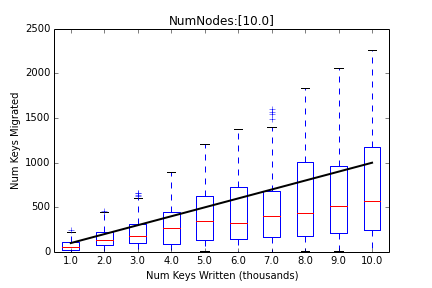
\includegraphics[scale=0.50]{10.png}
%\label{fig:subfigure10n}}
%
%\subfigure[Migration with 20 Nodes]{%
%  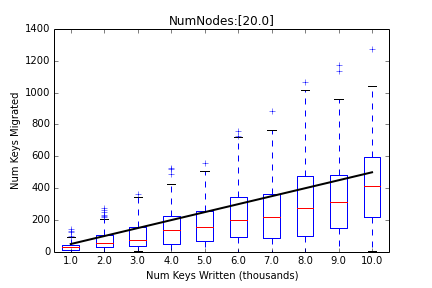
\includegraphics[scale=0.50]{20.png}
%\label{fig:subfigure20n}}
%
%\subfigure[Migration with 30 Nodes]{%
%  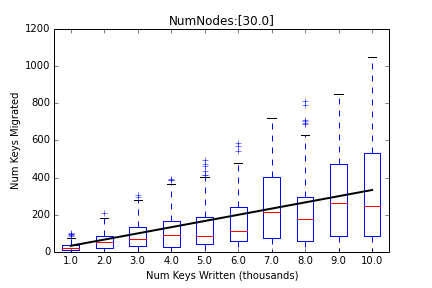
\includegraphics[scale=0.50]{30.png}
%\label{fig:subfigure30n}}
%
%\subfigure[Migration with 40 Nodes]{%
%  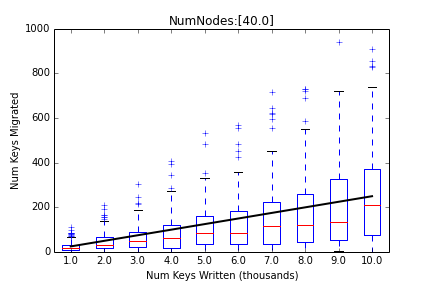
\includegraphics[scale=0.50]{40.png}
%  \label{fig:subfigure40n}}
%\label{fig:conhashing}
%\end{figure*}

\begin{figure}[hbt]
 \centering
 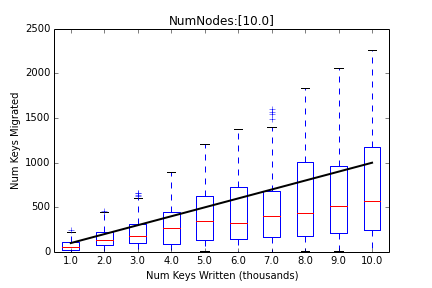
\includegraphics[scale=0.50]{10.png}
 \caption{Migration with 10 Nodes}
\label{fig:subfigure10n}
\end{figure}

\begin{figure}[hbt]
 \centering
 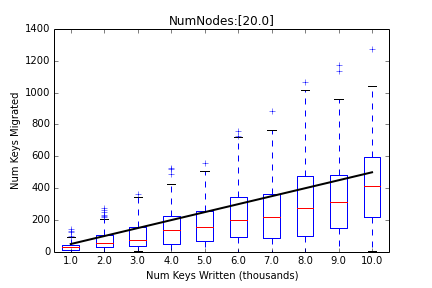
\includegraphics[scale=0.50]{20.png}
 \caption{Migration with 20 Nodes}
\label{fig:subfigure20n}}
\end{figure}

\begin{figure}[hbt]
 \centering
 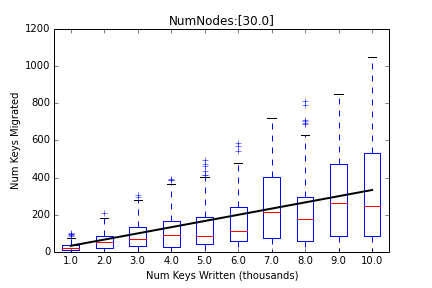
\includegraphics[scale=0.50]{30.png}
 \caption{Migration with 30 Nodes}
\label{fig:subfigure30n}
\end{figure}

\begin{figure}[hbt]
 \centering
 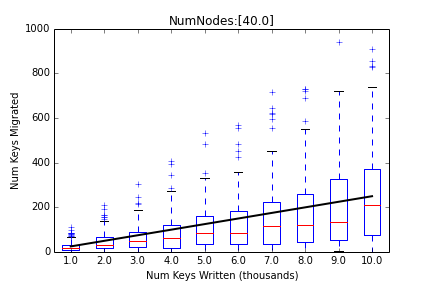
\includegraphics[scale=0.50]{40.png}
 \caption{Migration with 40 Nodes}
\label{fig:subfigure40n}
\end{figure}

Figure \ref{fig:conhashing} shows a box plot of number of keys that were migrated when a new node joins with a certain number of existing nodes and keys in the system with measurements from several runs of the experiment with the same initial conditions. For example, in figure \ref{fig:subfigure10n} the system had 10 nodes. We measured the number of keys that were migrated when an eleventh node joined the system. We generated keys at random and stored data in the system. The x-axis shows the number of keys that were in the system when the eleventh node joined the system. 

The black line shows the value of \(K/N\) where \(K\) is the number of keys in the system and \(N\) is the number of nodes in the system. The black line helps compare the performance of our consistent hashing scheme with our theoretical targets for the system described above. The number of key migrations is consistently below the black line. As expected the variability in the number of keys migrated reduced as the number of keys and the number of nodes in the system increases.

\section{Future Work} \label{futurework}
\begin{enumerate}
\item Sentinel support: The Redis Sentinel is designed to run in a configuration where there are multiple Sentinel processes cooperating together. The probability of false positives is lowered because multiple sentinels will detect failure and if the quorum which is the number of Sentinels that need to agree about the fact the master is not reachable, is present, a failover is authorized immediately as opposed to after a delay in the case of a single sentinel. A similar approach for DTSentinels can be used and handleJoin or handleLeave in case of a node joining or leaving can be triggered quickly. Also, DTSentinel here being the only sentinel, becomes the single point of failure. It is proved that at least three Sentinel instances are needed for a robust deployment**ref to sentinel page here** so that should be the minimum number of DTSentinels present as well. This would only make the system more fault tolerant but also would reduce the delay between server failure and its detection.

\item Improved logging mechanisms: Currently we use the logs to detect writes happening during migration. The incremental updates to the logs are used to find if there were any operations performed on the server. Better methods to obtain these increments would decrease the migration time. An approach that combines the Harp**ref to harp** method of logging along with timestamps to mark the actions, would suit our purpose as we would be able to extract operations that have occurred after a certain timestamp and apply them to the new server. Also, in case of synchronous writes to the backends, we could write to the log and have a background process update the primary and the backends.

\item Overhead related improvements: Python is a parsed language and is relatively slower than C. An implementation in a lower-level language would boost the system throughput as the processing time would decrease. Connection pools can be used to avoid reconnecting to the same server again.

\item serverCron() performs a number of periodic tasks for Redis, including verbose logging of database size and connected clients, resizing hash tables, closing idle/timed-out client connections, performing any post-background save or AOF rewrite cleanup, kicking off a background save if the save conditions as configured have been met, calculating LRU information and dealing with expired keys. All these features could be a valuable addition to DT. 
\end{enumerate}

\section{Conclusions} \label{conclusions}
conclusion and summary design here

\section{Acknowledgments} \label{acknowledgments}
future work here

\begin{thebibliography}{9}
\bibitem{chord} \emph{Chord: A Scalable Peer-toPeer Lookup Protocol for Internet Applications}  Ion Stoica, Robert Morris, David Liben Nowell, David R.Karger, M. Frans Kaashoek, Frank Dabek, and Hari Balakrishnan
\bibitem{redis} \emph{http://redis.io} Redis Documentation
\bibitem{harp} \emph{Replication in the Harp File System}  Barbara Liskov, Sanjay Ghemawat, Robert Gruber, Paul Johnson, Liuba Shrira, Michael Williams
\bibitem{conhash1} \emph{OceanStore: An architecture for global-scale persistent storage. In Proceedings of the Ninth international Conference on Architectural Support for Programming Languages and Operating Systems (Asplos 2000) (Boston, Ma, November 2000), Pp. 190-201} Kubiatowicz, J., Bindel, D., Chen, Y., Czerwinski, S.,
Eaton, P., Geels, D., Gummadi, R., Rhea, S.,Weatherspoon, H., Weimer, W., Wells, C., And Zhao, B.
\bibitem{conhash2} \emph{A scalable location service for geographic ad hoc routing. In Proceedings of the 6th ACM International Conference on Mobile Computing and Networking (Boston, Massachusetts, August 2000), pp. 120?130} Li, J., Jannotti, J., De Couto, D., Karger, D., And Morris,R.
\end{thebibliography}
{\small
\bibliographystyle{ieee}
\bibliography{egbib}
} 

\end{document}
